\begin{figure}[!t]
    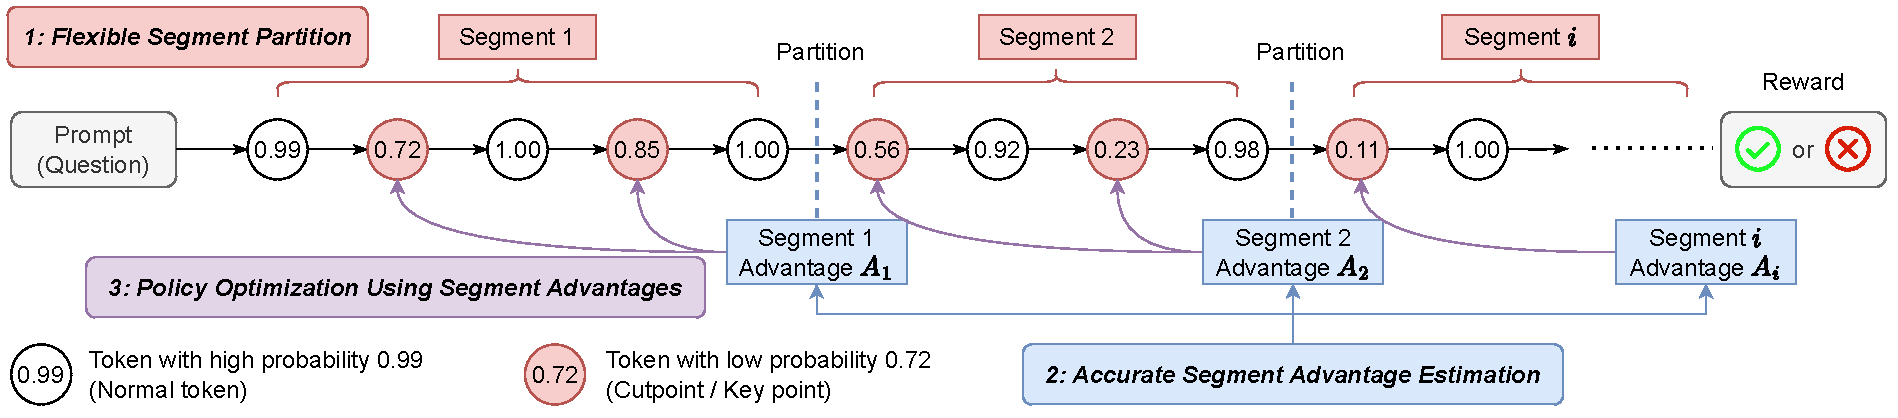
\includegraphics[width=\textwidth]{eval-figures/SPO-framework-short.pdf}
    \caption{Overview of SPO framework. Our framework consists of three components: segment partition, segment advantage estimation, and policy optimization, each of which can be implemented in different ways. This figure illustrates the cutpoint-based partition strategy used in SPO-chain, where partitioning occurs after a predetermined number of cutpoints. It also illustrates our probability-mask policy optimization method, which assigns the corresponding segment advantages specifically to the cutpoints instead of all tokens within a segment.}
    \label{fig:pipeline}
\end{figure}
\begin{figure}[!t]
    \centering
    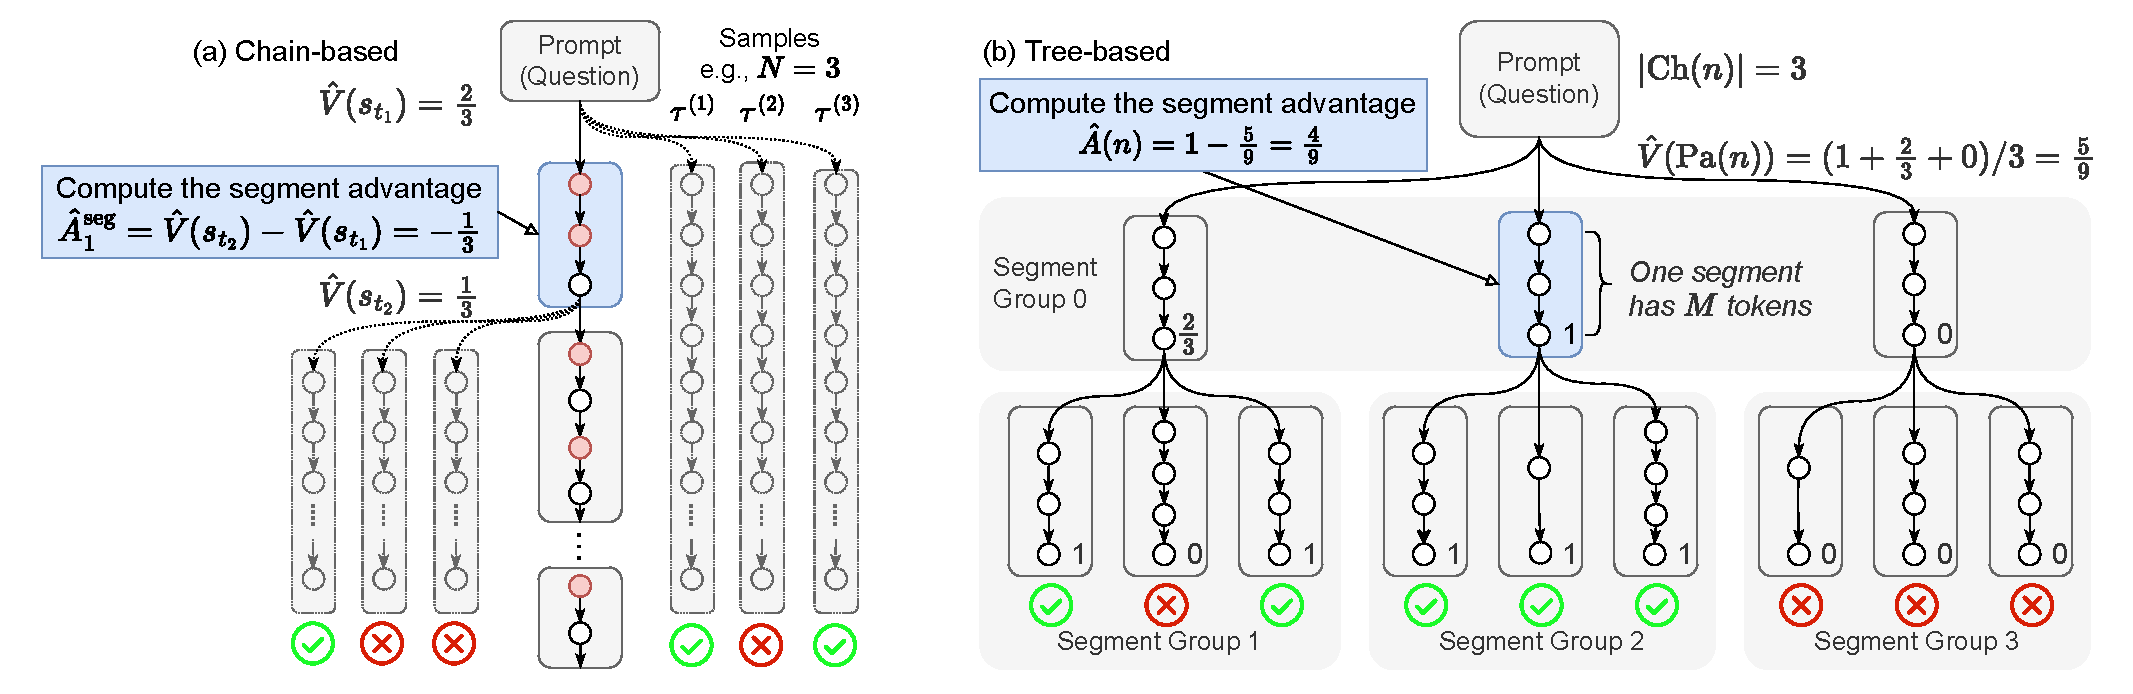
\includegraphics[width=\textwidth]{eval-figures/SPO-framework-both.pdf}
    \caption{\textbf{(a)} Chain-based advantage estimation method. For each segment, we independently sample \(N\) trajectories to estimate its value \(V\). The advantage for segment \(k\) is estimated as \(\hat V(s_{t_{k+1}})-\hat V(s_{t_k})\). \textbf{(b)} Tree-based advantage estimation method. Trajectories are organized in a tree structure, where nodes sharing the same parent form a group with identical prompts and token counts (except for leaf nodes, whose token lengths may vary). This hierarchical organization facilitates the calculation of advantages within each group.}
    \label{fig:sampling_method}
    \vspace{-0.6cm}
\end{figure}

\vspace{-0.2cm}
\section{Segment Policy Optimization}
\vspace{-0.2cm}

In this section, we introduce our segment policy optimization (SPO) framework. Effective credit assignment is crucial for training LLMs in reasoning tasks. Trajectory-level methods such as GRPO rely solely on sparse final rewards, making credit assignment challenging. Token-level methods like PPO heavily depend on the critic model, whose value estimation is often inaccurate. The SPO framework aims to balance these extremes by operating at the segment granularity, enabling richer feedback signals compared to GRPO and allowing more accurate Monte Carlo estimates of segment-level advantages, thereby bypassing the need for a critic model.

We develop the SPO framework guided by the following three challenging problems: \textbf{(1)} \textit{How to partition the generated sequence into multiple segments?} \textbf{(2)} \textit{How to accurately and efficiently estimate the advantage for each segment?} \textbf{(3)} \textit{How to update the policy by using the segment-level advantage?} The proposed SPO framework, as illustrated in Figure \ref{fig:pipeline}, adopts a modular architecture, where each of its components can be implemented using various strategies, allowing the framework to be tailored to diverse tasks and scenarios. In what follows, we introduce three key components of SPO to answer the above questions and further instantiate SPO with two instances, tailored for short and long CoT scenarios.

\textbf{(1) Flexible Segment Partition.} A segment is defined as a contiguous sequence of generated tokens, denoted as \(\text{seg}_k = [y_{t_k}, y_{t_k+1}, \dots, y_{t_{k+1}-1}]\), where \(t_k\) is the starting token index of the \(k\)-th segment.  Formally, given a full generated trajectory \(\boldsymbol y = [y_1, y_2, \dots, y_T]\),  the partition can be expressed as \(\boldsymbol y = [y_1, y_2, \dots, y_T]=[\text{seg}_1,\text{seg}_2,\cdots,\text{seg}_K]\). The SPO framework supports arbitrary partition strategies, allowing flexible definition of segment boundaries, without requiring semantic completeness. This flexibility enables us to choose partition granularity between token-level and trajectory-level, allowing a trade-off between computational cost and credit assignment. In this work, we consider two main partition strategies, designed for different scenarios: \textbf{(a) Fixed Token Count Partition:} A straightforward strategy that divides the sequence into segments of a predetermined fixed number of tokens. \textbf{(b) Adaptive Cutpoint-based Partition:} An advanced strategy (see Section \ref{subsec:segment-partition-based-on-fixed-cutpoint-intervals}) that defines segments by accumulating a fixed number of low probability tokens (i.e., tokens whose probabilities $\pi_\theta(y_t|s_t)$ are less than a threshold $\rho$). This strategy places segment boundaries at positions where \( V \) values are more likely to change, avoiding the issue in the fixed token count partition strategy where \( V \) values may remain unchanged between segment boundaries when each segment is short.

\textbf{(2) Segment Advantage Estimation via Monte Carlo.} 
After obtaining each segment \(\text{seg}_k= [y_{t_k}, y_{t_k+1}, \dots, y_{t_{k+1}-1}]\), we define the segment advantage in the following way:
\begin{equation}
\label{eq:segA}
A_k^{\mathrm{seg}} := V(s_{t_{k+1}}) - V(s_{t_k})= V([\boldsymbol x,\text{seg}_1,\dots, \text{seg}_{k}]) - V([\boldsymbol x,\text{seg}_1,\dots, \text{seg}_{k-1}]),    
\end{equation}
which measures the incremental improvement in expected reward resulting from generating the tokens in \(\text{seg}_k\). The core challenge lies in accurately estimating the value function \(V(s)\). A common approach is to train a critic model. However, in the LLM scenario, critic-based methods struggle to produce accurate state-value estimates due to large variations across prompts and limited trajectory data per prompt, as empirically illustrated by \cite{kazemnejad2024vineppounlockingrlpotential}. Given these considerations, we propose to bypass the critic entirely and instead adopt Monte Carlo (MC) estimation to compute unbiased estimates of segment values directly from sampled trajectories. While high variance is often a concern with MC estimation, in the LLM setting, rewards are typically sparse and binary, significantly mitigating the variance issue. Specifically, we can view \( V \) as a Bernoulli variable, and the MC variance is at most \( 0.25 \). We find that the accuracy obtained with a small number of samples (\( N=4\) or \( N=9 \)) is sufficient for effective policy optimization. Our SPO framework supports various MC sampling strategies: \textbf{(a) Chain-based Advantage Estimation:} Independently roll out \(N\) trajectories from state \( s \), and estimate \( V(s) \) as the average reward of these trajectories, further yielding the estimation of the advantage $A_k^{\mathrm{seg}}$ following Equation \eqref{eq:segA}. \textbf{(b) Tree-based Advantage Estimation:} An advanced strategy of advantage estimation for improved sample efficiency (see details in Section \ref{subsec:tree-like-segment-advantage-estimation}).  Unlike the chain-based advantage estimation, which discards MC samples after estimating the $V$ values, this strategy organizes MC samples into a tree structure and computes the $V$ values via bottom-up aggregation of rewards along the tree. Nodes sharing the same parent have identical prompts and token counts, forming segment groups, enabling advantage computations within each group. This tree structure allows the reuse of MC samples for policy optimization, significantly enhancing sample efficiency in the long CoT scenario.

\textbf{(3) Policy Optimization Using Segment Advantages.}
Given a set of generated segments \(\{\text{seg}_k\}\) and their corresponding advantages \(\{A_k^{\mathrm{seg}}\}\), we now focus on effectively leveraging training samples to update the policy \(\pi_{\theta}\). Specifically, we can adapt various policy optimization approaches into our SPO framework: \textbf{(a) Policy Gradient:} We can assign \( A_k^{\mathrm{seg}} \) to all tokens contained within the $k$-th segment \(\text{seg}_k\) and then optimize using the PPO loss; \textbf{(b) Policy Gradient with Token-Probability Masks:} An improved version of policy gradient (see details in Section \ref{subsec:policy-optimization-using-ppo-loss-with-prob-mask}), incorporating probability masks. Instead of uniformly assigning \( A_k^{\mathrm{seg}} \) to all tokens within the segment, this strategy exclusively assigns \( A_k^{\mathrm{seg}}\) only to low-probability tokens, based on the intuition that these tokens primarily contribute to the segment's advantage. This refined approach further enhances the credit assignment to critical tokens; \textbf{(c) Other Strategies:} Our framework can also be adapted to other policy optimization methods such as policy iteration-based approach (see discussions in Appendix \ref{appendix:policy_iteration}) and potentially GFlowNet-based optimization \cite{bartoldson2025trajectorybalanceasynchronydecoupling}.